\documentclass{manual}
\pagenumbering{gobble}

\title{Dual Low-Current Galvanostat}
\author{Blaise Thompson}

\begin{document}

\maketitle

\vspace*{\fill}
\begin{center}
  \includegraphics[width=0.75\linewidth]{../pictures/2018-11-14_104721}
\end{center}
\vspace*{\fill}

\section{Overview \& Performance}
\pagenumbering{arabic}

The dual galvanostat is designed to force a small, constant current through an electrolytic cell.
The voltage floats to whatever is needed to maintain that current.
The maximum rated output voltage is 13 V, although in practice the voltage may be able to float several hundred millivolts above 13.
The positive output (red) is guaranteed to be greater than or equal to the negative return (black), in voltage.
Each output of the dual galvanostat is independent, such that the applied voltages may be different.
However, the current set-point of both outputs is the same.

The dual galvanostat is designed to deliver relatively small currents accurately.
These small current set-points can be crucial when driving particularly slow reactions.
When a galvanostat is set to a current that the reaction of interest cannot support, the galvanostat will naturally swing the output voltage higher.
Often, the galvanostat will end up driving higher-potential undesirable reactions that are more kinetically favorable.
For this reason, this galvanostat has been designed to hold current set-points between 10 $\mu$A and 9.99 mA.

\autoref{fig:setpoint} shows the agreement between the set current and actual measured current for a constant load of 100 $\Omega$.
Note that the data is displayed on a log-log plot.
The output and setpoint agree to within measurement error for all setpoints above 0.30 mA.
Below this setting, however, the agreement worsens---the measured current consistently overshoots the set current.
The absolute deviation between setpoint and measured current never exceeds 30 $\mu$A.
Please note that the galvanostat is still capable of maintaining these low currents.
The displayed value simply may not correspond to the actual current, so an independent calibration is warranted.

\autoref{fig:load} shows the applied voltage as a function of load resistance.
In all cases, the set current was 1 mA.
The grey line shows ``ideal'' ohms law behavior.
The saturation of the galvanostat at roughly 13 V can easily be seen.

\clearpage
\begin{figure}
  \includegraphics[width=\linewidth]{../data/2018-11-13/setpoint}
  \caption{
    Measured current versus set current.
    On this log-log plot, the entire set-point range of 10 $\mu$A to 9.99 mA can clearly be seen.
    For both outputs, agreement within measurement error is achieved from 0.30 mA to 9.99 mA.
    Unfortunately, both outputs become nonlinear at the lowest setpoints, systematically overshooting the desired current.
    For an unknown reason, the agreement is worse for the left-hand output.
    All readings were taken with a load of 100 $\Omega$.
  }
  \label{fig:setpoint}
\end{figure}
\clearpage

\clearpage
\begin{figure}
  \includegraphics[width=\linewidth]{../data/2018-11-14/load}
  \caption{
    Measured applied voltage versus load resistance.
    All readings were taken at a current set-point of 1 mA.
    The ``ideal'' ohms law behavior is represented by the grey diagonal line.
    Both outputs saturate at just above 13 V.
  }
  \label{fig:load}
\end{figure}
\clearpage

\section{Troubleshooting}

This section describes calibration and testing of the dual galvanostat.

When troubleshooting or inspecting the circuit, start by testing each of the power test points.
All power voltages should be measured relative to circuit common at test point 1.
TP2 should be +15 V.
TP5 should be -6 V.
If these are not maintained, check the regulator U1, the inverter U4, and the capacitors C1, C2, C3, C4, \& C5.
C4 and C5 are electrolytic, so they may be the most suspect.

There are three board-level trimpots that can be adjusted to calibrate the output of the dual galvanostat.
Refer to the schematic and board drawings at the end of this manual to find the location of these trimpots.
They are all three Bourns 3296 series, blue boxes with brass adjusts on the top.

The first trimpot, RV4, is located near the top of the PCB.
Adjust this trimpot while monitoring the voltage at TP6 relative to circuit common (TP1).
Adjust the external digipot (RV3), and ensure that the voltage at TP6 corresponds directly to the setting of RV3, in mV.
For example, when RV3 reads 999, the voltage at TP6 should be 0.999 V.
Typically it is best to adjust this pot with RV3 set to a large number, since this gives you the most sensitivity in defining the necessary proportionality.

You may find that TP6 does not respond, or that the response is not proportional to the setting of RV3.
In this case, there may be a problem with the differential amplifier U5 or with the dual buffer U3.
Test the voltage difference between TP3 and TP4, noting that TP3 is always equal to or more positive than TP4.
Like TP6, the voltage between these test points should correspond to the setting of RV3, in mV.
If you are able to confirm correct behavior at TP3 \& TP4 but not at TP6, start by verifying power and replacing U3 and U5.

Both outputs of the dual galvanostat are driven directly by U6, a dual op-amp.
Each of these has a separate trim pot for the current control, RV1 and RV2.
After verifying correct behavior with at TP6, use a current meter placed across each output to calibrate the control resistors.
Again, it is recommended to adjust these trim pots with RV3 set to a large number.

\section{Appendix}

This appendix contains the following:
\begin{ditemize}
  \item parts list
  \item circuit schematic
  \item full board
  \item top layer
  \item bottom layer
\end{ditemize}

\clearpage
\subsection{Parts}

Parts list.
Costs are approximate.
Trivial components like screws, standoffs, feet are not included.

\begin{tabular}{
    P{\dimexpr 0.02\linewidth-2\tabcolsep}|
    p{\dimexpr 0.3\linewidth-2\tabcolsep}|
    p{\dimexpr 0.37\linewidth-2\tabcolsep}|
    p{\dimexpr 0.15\linewidth-2\tabcolsep}|
    P{\dimexpr 0.15\linewidth-2\tabcolsep}}
  & name & part & vendor & cost (USD) \\ \hline
  1 & enclosure & CU-3005-A:BUD & UW Stock & 9.00 \\
  1 & barrel plug, 2.1 mm & 722A:SWITCHCRAFT & UW Stock & 3.00 \\
  1 & switch &  R1966ABLKBLKEFGRN:E-SWITCH & UW Stock & 2.00 \\
  1 & black banana & 108-0902-001:CINCH & UW Stock & 0.75 \\
  1 & red banana & 108-0903-001:CINCH & UW Stock & 0.75 \\ \hline
  1 & R1 & resistor, 1 k$\Omega$, 1/4 W & UW Stock & 0.00 \\
  2 & R2, R3 & resistor, 240 $\Omega$, 1/4 W & UW Stock & 0.00 \\
  2 & RV1, RV2 & 2K-3296:BOURNS & UW Stock & 3.00 \\
  1 & RV3 & 3683S-1-103L:BOURNS & UW Stock & 10.00 \\
  1 & RV4 & 100K-3296:BOURNS & UW Stock & 3.00 \\ \hline
  1 & C1 & capacitor, tantalum, 10 $\mu$F & UW Stock & 0.25 \\
  1 & C2 & capacitor, tantalum, 330 nF & UW Stock & 0.25 \\
  1 & C3 & capacitor, tantalum, 100 nF & UW Stock & 0.25 \\
  2 & C4, C5 & capacitor, electrolytic, 10 $\mu$F & UW Stock & 0.10 \\ \hline
  4 & J0, J1, J2, RV3 (pins) & 22-23-2021:MOLEX & UW Stock & 0.25 \\
  4 & J0, J1, J2, RV3 (socket) & 22-01-3027:MOLEX & UW Stock & 0.25 \\ \hline
  1 & TP1 & 5012:KEYSTONE & UW Stock & 0.50 \\
  1 & TP2 & 5010:KEYSTONE & UW Stock & 0.50 \\
  1 & TP5 & 5011:KEYSTONE & UW Stock & 0.50 \\
  3 & TP3, TP4, TP6 & 5014:KEYSTONE & UW Stock & 0.50 \\ \hline
  5 & 8 pin DIP socket & 110-93-308-41-001000:MILL-MAX & UW Stock & 1.00 \\
  1 & U1 & L7815CV:STM & UW Stock & 0.50 \\
  1 & U4 & LMC7660IN/NOPB:TI & \href{https://www.digikey.com/product-detail/en/texas-instruments/LMC7660IN-NOPB/LMC7660IN-NOPB-ND/32523}{DigiKey} & 1.50 \\
  1 & U5 & INA105KP:TI & \href{https://www.digikey.com/product-detail/en/texas-instruments/INA105KP/INA105KP-ND/251073}{DigiKey} & 10.00 \\
  3 & U2, U3, U6 & LM358P:TI & \href{https://www.digikey.com/product-detail/en/texas-instruments/LM358P/296-1395-5-ND/277042}{DigiKey} & 0.50 \\
\end{tabular}

\includepdf[angle=-90, fitpaper=true]{../PCB/schematic.pdf}
\includepdf[angle=-90, fitpaper=true]{../PCB/pcb.pdf}
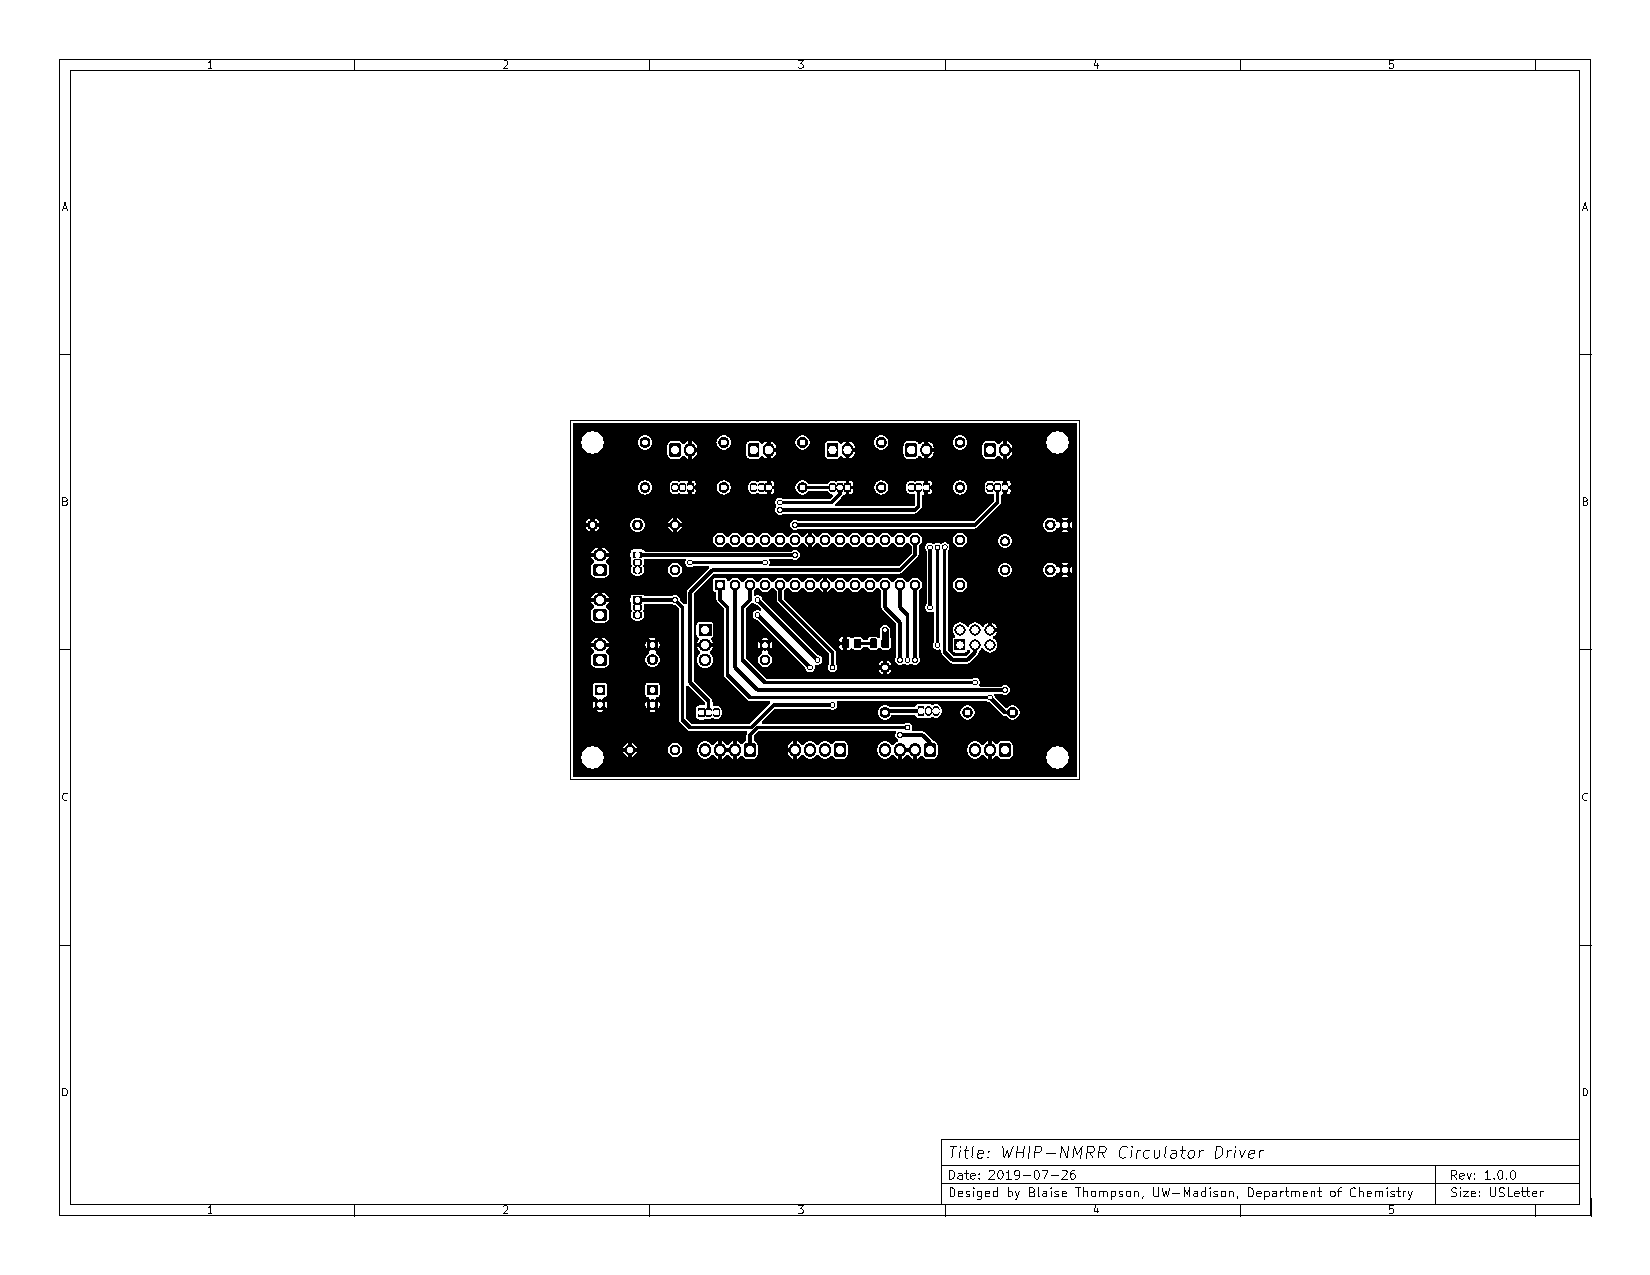
\includepdf[angle=-90, fitpaper=true]{../PCB/front.pdf}
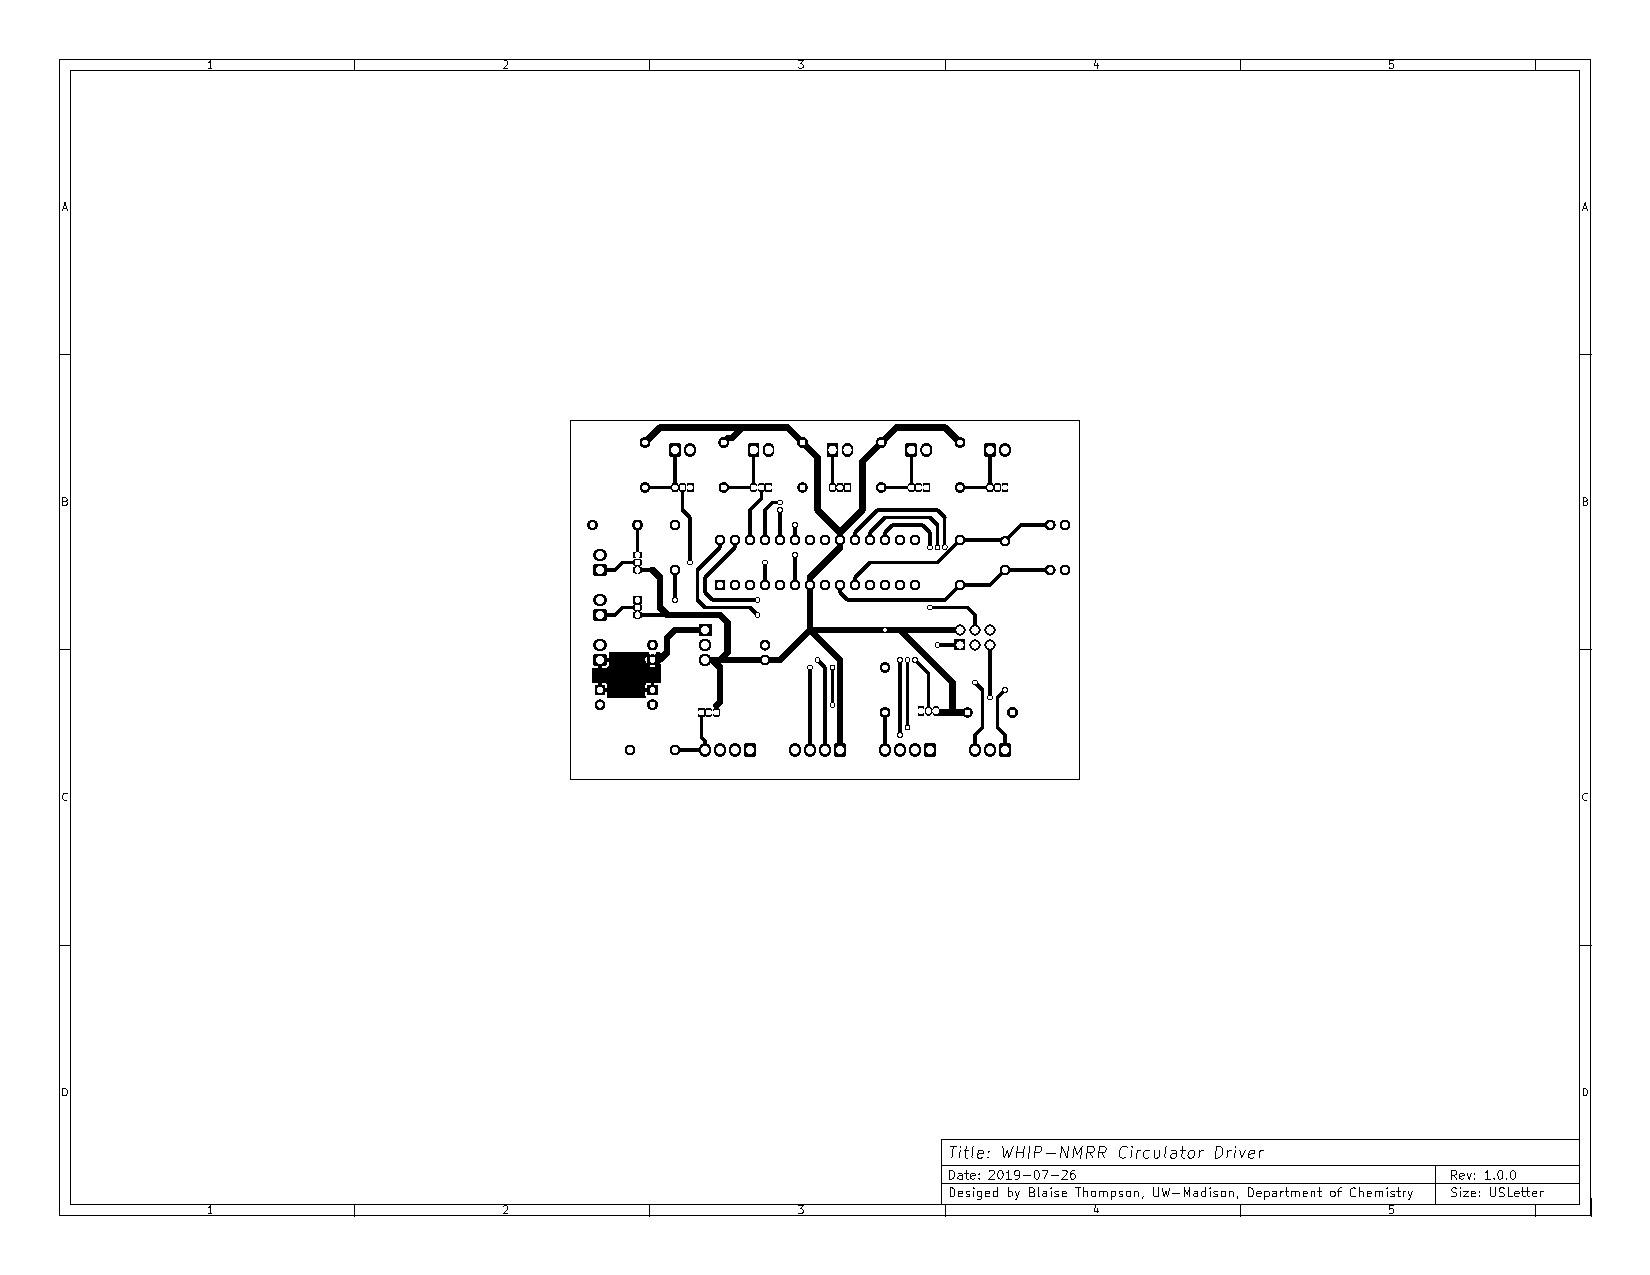
\includepdf[angle=-90, fitpaper=true]{../PCB/back.pdf}

\end{document}
